\documentclass[14pt, a5paper, twoside, extrafontsizes]{memoir}

\usepackage{lettrine}

% indentation of the first word on the first line after the drop capital
\setlength{\DefaultFindent}{6pt}

% extra indentation for the first word on the next line
\setlength{\DefaultNindent}{0pt}

\renewcommand*{\DefaultLoversize}{-.2}
\renewcommand*{\DefaultLraise}{.6}
\renewcommand{\LettrineTextFont}{\relax}

\renewcommand*{\LettrineFont}{%
 \LettrineFontHook
 \fontsize{18pt}{18pt}%
 \selectfont
}

% \leadword{first word [to be enlarged]}{second word}
\newcommand{\leadword}[2]{%
  \lettrine[realheight=true]{#1}{#2}
}


\usepackage{graphicx}
\usepackage{pgffor}
\usepackage{anysize}
\usepackage[all]{nowidow}
\usepackage{relsize}
\usepackage{ragged2e}

\usepackage[pdfauthor={יהודה הנשיא},
  pdftitle=\sederTitle,
  pdfsubject={תורה שבעל פה},
  pdfproducer={סיימון מונטגיו, הוצאת חטף סגול},
  pdfdirection=R2L,
  pdfcreator=xelatex,
  colorlinks=false, linkcolor=blue,
  linkbordercolor={.6 .6 .6},
  plainpages=true]{hyperref}
\makeatletter
\Hy@AtBeginDocument{%
  % Override border definition set with colorlinks=true
  \def\@pdfborder{0 0 1}
  % Overrides border style set with colorlinks=true
  % Hyperlink border style will be underline of width 1pt
  \def\@pdfborderstyle{/S/U/W 1}
}
\makeatother

\usepackage{polyglossia}
\setmainlanguage[numerals=hebrew]{hebrew}
\setmainfont{SBL Hebrew}
\setotherlanguage{english}

% General formatting
\marginsize{1.2in}{.8in}{.5in}{.5in}
\renewcommand{\baselinestretch}{1.1}
\parskip 8pt
\parindent 0pt
\makeevenhead{myheadings}{\thepage}{}{\texthebrew{\sederTitle}}
\makeoddhead{myheadings}{\texthebrew{\tractateTitle}}{}{\thepage}
\makepagestyle{mytitlepage}

\newcounter{perekCount}
\newcounter{halachaCount}[perekCount]
\newcounter{tractateCount}
\newcounter{perakim}

% \tractatehead{title for printing}{hyperlink reference}
\newcommand{\tractatehead}[2]{%
 \cleardoublepage
 \setcounter{perekCount}{0}
 \thispagestyle{empty}
 \def \tractateTitle{#1}
{\centering\LARGE\bfseries \hypertarget{#2}{#1}

  }}

% \summarycontentsline{tractate name}{hyperlink reference}
%                     {number of chapters [numeric]}
\newcommand{\summarycontentsline}[3]{%
\setcounter{perakim}{#3}%
\stepcounter{tractateCount}%
\textlarger{\alph{tractateCount}} \hyperlink{#2}{#1} \alph{perakim} פרקים\hdot%
}

\newcommand{\summarycontents}[1]{
  \centerlastline
  \foreach \linkText / \linkName / \numChapters in #1 {
      \summarycontentsline{\linkText}{\linkName}{\numChapters}
  } 
}

% \sederContents{number of tractates [hebrew]}
%               {list of tractates}{total number of chapters [hebrew]}
\newcommand{\sederContents}[3]{
  {
    \centering
    {\Large משניות \sederTitle}

  יש בו #1 מסכתות וזהו סדורן

    \begin{minipage}{0.9\textwidth}
    \small
    \summarycontents{#2}

    בין הכל \textlarger[2]{#3} פרקים׃
    \end{minipage}

  }
}

% centered rubric
\newcommand{\crubric}[1]{{\centering\small\bfseries{#1}

  }}

% centered header (keep with next paragraph)
\newcommand{\chead}[1]{%
  \vspace{0.25em}
  \needspace{4\baselineskip}
  \crubric{#1}
}

% centered footer
\newcommand{\cfoot}[1]{%
  \vspace{0.25em}
  \crubric{#1}
}

\newcommand{\mispar}[1]{{\footnotesize\textsuperscript{\alph{#1}}}}

% There is no Unicode character for the raised dot used in many Hebrew books
% as mid-sentence punctuation. This is a hack to replace it using
% U+005C4 HEBREW MARK UPPER DOT
\sfcode`\^^^^05c43000
\newcommand{\hdot}{\raisebox{-0.5\height}{^^^^2009^^^^2009^^^^05c4} }

\tolerance=8192

% \perek{first word}{rest of first halacha}
% First halacha in a perek
\newcommand{\perek}[2]{%
 \stepcounter{perekCount}
 \perekbar{פרק \alph{perekCount}}{#1}{#2}
}

% \baraita[subhead]{first word}{rest of first halacha}
% First halacha in a baraita (e.g. after the last perek of Bikkurim)
\newcommand{\baraita}[3][]{%
 \setcounter{halachaCount}{0}
 \perekbar[#1]{ברייתא}{#2}{#3}
}

% \perekbar[subhead]{heading}{first word}{rest of first halacha}
% Called by \perek and \baraita
\newcommand{\perekbar}[4][]{%
 \vspace{0.5em}
 \stepcounter{halachaCount}
 \needspace{2\baselineskip}
 \crubric{#2}

 \centerlastline
 #1

 \leadword{#3}#4
}

% \halacha{text}
% Prints a halacha
\newcommand{\halacha}[1]{%
 \stepcounter{halachaCount}
 \mispar{halachaCount}
 \centerlastline
 #1\nowidow
}

\newcommand{\selik}{~~{\footnotesize סליק}}

% \titlepage{Hebrew chronogram for year of issue}
%           {Gregorian year of issue}
\newcommand{\titlepage}[2]{%
\Centering

  {\huge\bfseries משניות}

  {\LARGE\bfseries\sederTitle}

  \vspace{1em}

  \vspace{0.5em}
  על פי מהדורת הרב דוד אלטאראס ז״ל\\שהודפס בשנת ה׳תק״ע בעיר פיסא

    \vspace{8em}
    פה {\LARGE ירושלים} יע״א

    {\small שנת} #1 {\small לפ״ק}

    \vspace{2em}
      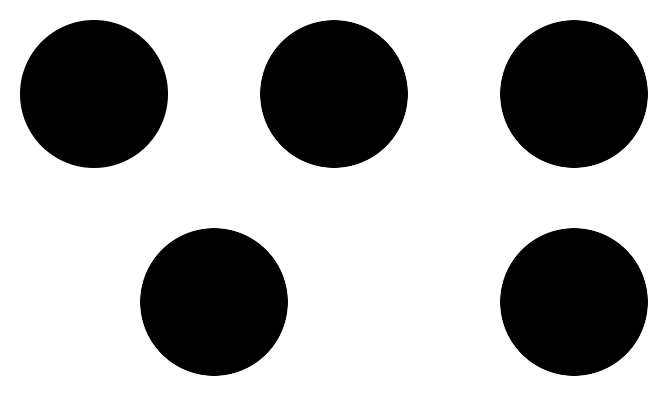
\includegraphics[width=10mm]{hatafSegolLogoNoText.png}\\

    \vspace{.5em}
  {
    \bfseries הוצאת חטף־סגול\\#2

 {\footnotesize  הובא לדפוס באמצעות \XeLaTeX\ ע״י שמעון מונטגיו}

  }

}

% code for special handling of specific numbers by "Circumscribe" copied from https://tex.stackexchange.com/questions/300008/modify-specific-hebrew-alpha-numerals-on-page-number
% with a few modifications to the function names
\makeatletter
\let\@hebrew@numeral@usual\@hebrew@numeral  %% <- store old definition
\newcommand*\@hebrew@numeral@special[1]{%   %% <- new definition
  \ifcsdef{specialnum@\number#1}            %% <- if this number is listed
    {\csuse{specialnum@\number#1}}          %% <- give it special handling
    {\@hebrew@numeral@usual{#1}}%           %% <- otherwise use usual handling
}
\let\@hebrew@numeral\@hebrew@numeral@special %% <- replace old definition
\makeatother

%% Declare numbers for special handling:
\newcommand*\newspecialnum[2]{\csdef{specialnum@#1}{#2}}
\newspecialnum{16}{יו}    % At least some Livorno printings don't use טז for 16
\newspecialnum{116}{קיו}
\newspecialnum{216}{ריו}
\newspecialnum{316}{שיו}
\newspecialnum{416}{תיו}
\newspecialnum{516}{תקיו}
\newspecialnum{616}{תריו}
\newspecialnum{716}{תשיו}
\newspecialnum{816}{תתיו}
\newspecialnum{916}{תתקיו}
\newspecialnum{18}{חי}    % Add some other "specials" while we're here
\newspecialnum{270}{ער}
\newspecialnum{272}{ערב}
\newspecialnum{275}{ערה}



\def \shiurTitle{מסכת ברכות}
\marginsize{1.2in}{.8in}{.5in}{.5in}
\renewcommand{\baselinestretch}{1.1}

\begin{document}
\frontmatter
\pagestyle{myheadings}
\thispagestyle{mytitlepage}
\begin{hebrew}
{\centering  

  {\huge\bfseries משניות}
  
  {\LARGE\bfseries סדר זרעים}

  \vspace{1em}
    ולע״ע ליוקר מציאותן נדפסו ביתר שאת ובהגהה
  מזוקקת שבעתים על ידי מדקדקים זהירים ובקיאים
  במלאכת שמים ישלח עזרתו מקדש וחיינו מיומים׃

  \vspace{
    0.5em}
  על פי מהדורת הרב דוד אלטאראס ז״ל\\שנת ה׳תרכ״ה ליוורנו
  
    \vspace{3.5em}
  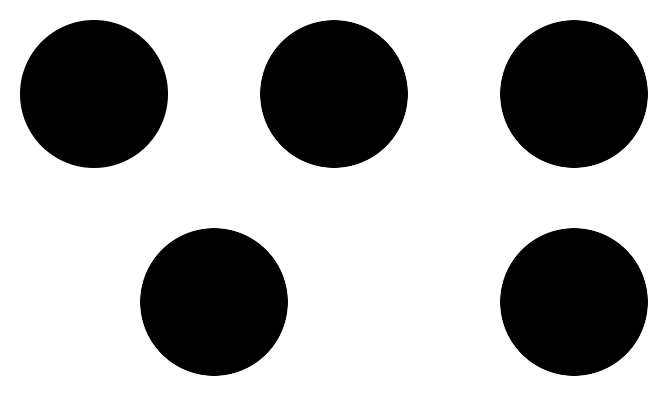
\includegraphics[width=12mm]{hatafSegolLogoNoText.png}\\
  
    \vspace{.5em}
  {
    \bfseries הוצאת חטף־סגול\\2021
    
 {\footnotesize  הובא לדפוס באמצעות \XeLaTeX\ ע״י סיימון מונטגיו}

  }

    \vspace{1em}
    פה {\LARGE ירושלים} יע״א

    {\small שנת}
    ונתתי בציון
    {\Large תׄשׄוׄעׄהׄ}
    {\small לפ״ק}
    
}

\mainmatter
\cleardoublepage
\thispagestyle{empty}
\bighead{מסכת ברכות}
\sechead{יום א}

\halachaa[688]{א}{מֵאֵימָתַי}{קוֹרִין}{
אֶת שְׁמַע בְּעַרְבִית\hdot
מִשָּׁעָה שֶׁהַכֹּהֲנִים נִכְנָסִים לֶאֱכוֹל בִּתְרוּמָתָן\hdot
עַד סוֹף הָאַשְׁמוֹרֶת הָרִאשׁוֹנָה\hdot
דִּבְרֵי רִבִּי אֱלִיעֶזֶר\hdot
וַחֲכָמִים אוֹמְרִים עַד חֲצוֹת\hdot
רַבָּן גַּמְלִיאֵל אוֹמֵר\hdot
עַד שֶׁיַּעֲלֶה עַמּוּד הַשַּׁחַר\hdot
מַעֲשֶׂה שֶׁבָּאוּ בָנָיו מִבֵּית הַמִּשְׁתֶּה\hdot
אָֽמְרוּ לוֹ\hdot
לֹא קָרִינוּ אֶת שְׁמַע\hdot
אָמַר לָהֶם\hdot
אִם לֹא עָלָה עַמּוּד הַשַּׁחַר\hdot
חַיָּיבִין אַתֶּם לִקְרוֹת\hdot
וְלֹא זוֹ בִלְבַד\hdot
אֶלָּא כָּל מַה שֶּׁאָֽמְרוּ חֲכָמִים עַד חֲֲצוֹת\hdot
מִצְוָתָן עַד שֶׁיַּעֲלֶה עַמּוּד הַשַּׁחַר\hdot
הֶקְטֵר חֲֲלָבִים וְאֵבָרִים\hdot
מִצְוָתָן עַד שֶׁיַּעֲלֶה עַמּוּד הַשַּׁחַר\hdot
וְכָל הַנֶּאֱכָלִים לְיוֹם אֶחָד\hdot
מִצְוָתָן עַד שֶׁיַּעֲלֶה עַמּוּד הַשַּׁחַר\hdot
אִם כֵּן לָמָּה אָֽמְרוּ חֲכָמִים עַד חֲצוֹת\hdot
כְּדֵי לְהַרְחִיק אֶת הָאָדָם מִן הָעֲבֵירָה׃
}

\halacha{ב}{
מֵאֵימָתַי קוֹרִין אֶת שְׁמַע בְּשַׁחְרִית
מִשֶׁיַּכִּיר בֵּין תְּכֵלֶת לְלָבָן\hdot
רִבִּי אֱלִִיעֶזֶר אוֹמֵר בֵּין תְּכֵלֶת לְכַרְתִּי (וְגוֹמְרָהּ) עַד הֵנֵץ הַחַמָּה\hdot
רִבִּי יְהוֹשֻׁעַ אוֹמֵר\hdot
עַד שָׁלֹשׁ שָׁעוֹת\hdot
שֶׁכֵּן דֶּרֶךְ בְּנֵי מְלָכִים\hdot
לַעֲמוֹד בְּשָׁלֹשׁ שָׁעוֹת\hdot
הַקּוֹרֵא מִכָּאן וְאִילָךְ\hdot
לֹא הִפְסִיד\hdot
כְּאָדָם הַקּוֹרֵא בַּתּוֹרה׃
}

\halacha{ג}{
בֵּית שַׁמָּאי אוֹמְרִים בָּעֶרֶב כָּל אֶָדָם יַטּוּ וְיִקְרְאוּ\hdot
וּבַבֹּקֶר יַעַמְדוּ שֶׁנֶּאֱמַר וּבְשָׁכְבְּךָ ובְקוּמֶךָ\hdot
וּבֵית הִלֵּל אוֹמְרִים כָּל אָדָם קוֹרֵא כְדַרְכּוֹ\hdot
שֶׁנֶּאֱמַר וּבְלֶכְתְּךָ בַדֶּרֶךְ\hdot
אִם כֵּן לָמָּה נֶאֱמַר וּבְשָׁכְכְּךָ וּבְקוּמֶךָ\hdot
(אֶלָּא)
בְּשָׁעָה שֶׁדֶּרֶךְ בְּנֵי אָדָם שׁוֹכְבִים וּבְשָעֶָה שֶׁדֶּרֶךְ בְּנֵי אָדָם עוֹמְדִִים\hdot
אָמַר רִבִּי טַרְפוֹן\hdot
אֲנִי הָיִיתִי בָּא בַדֶרֶךְ\hdot
וְהִטֵּתִי לִקְרוֹת כְּדִבְרֵי בֵית שַׁמָּאי\hdot
וְסִכַּנְתִּי בְעַצְמִי\hdot
מִפְּנֵי הַלִּסְטִים\hdot
אָֽמְרוּ לוֹ כְּדַי הָיִיתָ לָחוֹב בְּעַצְמָךְ שָׁעָבַרְתָּ עַל דִּבְרֵי בֵית הִלֵּל׃
}

\halacha[1147]{ד}{
בַּשַּׁחַר מְבָרֵךְ שְׁתַּיִם לְפָנֶיהָ\hdot
וְאַחַת לְאַחֲרֶיהָ\hdot
וּבָעֶרֶב מְבָרֵךְ שְׁתַּיִם לְפָנֶיהָ\hdot
וּשְׁתַּיִם לְאַחֲרֶיהָ\hdot
אַחַת אֲרֻכָּה וְאַחַת קְצָרָה\hdot
מָקוֹם שָאָֽמְרוּ לְהַאֲרִיךְ אֵינוֹ רַשָׁאי לְקַצֵּר\hdot
לְקַצֵּר אֵינוּ רַשָׁאי לְהַאֲרִיךְ\hdot
לַחֲתוֹם אֵינוֹ רַשָּאי שֶׁלֹּא לַחֲתוֹם\hdot
וְשֶׁלֹּא לַחֲתוֹם אֵינוֹ רַשָּׁאי לַחֲתוֹם׃
}

\halacha[638]{ה}{
מַַַַַַַזְכִּירִין יְצִיאַת מִצְרַיִם בַּלֵּילוֹת\hdot
אָמַר רִבִּי אֶלְעָזָר בֶּן עֲזַרְיָה הֲרֵי אֲנִי כְּבֶן שִׁבְעִים שָׁנָה וְלֹא זָכִיתִי שֶׁתֵּאָמֵר יְצִיאַת מִצְרַיִם בַּלֵּילוֹת\hdot
עַד שֶׁדְּרָשָׁהּ בֶּן זוֹמָא\hdot
שֶׁנֶּאֱמַר לְמַעַן תִּזְכּוֹר אֶת יוֹם צֵאתְךָ מֵאֵרֶץ מִצְרַיִם כֹּל יְמֵי חַיֶּיךָ\hdot
יְמֵי חַיֶּיךָ הַיָּמִים\hdot
כֹּל יְמֵי חַיֶּיךָ הַלֵּילוֹת\hdot
וַחֲכָמִים אוֹמְרִים יְמֵי חַיֶּיךָ הָעוֹלָם הַזֶּה\hdot
כֹּל יְמִֵי חַיֶּיךָ לְהָבִיא לִימוֹת הַמָּשִׁיחַ׃
}

\halachaa[185]{ב}{הָיָה}{קוֹרֵא}{בַתּוֹרָה\hdot
וְהִגִּיעַ זְמַן הַמִּקְרָא\hdot
אִם כִּוֵּין לִבּוֹ יָצָא\hdot
וְאִם לָאוּ לֹא יָצָא\hdot
בַּפְּרָקִים שׁוֹאֵל מְפְּנֵי הַכָּבוֹד וּמֵשִׁיב\hdot
וּבָאֶמְצַע שׁוֹאֵל מִפְּּנֵי הַיִּרְאָה וּמֵשִׁיב\hdot
דִּבְרֵי רִבִּי מֵאִיר\hdot
רִבִּי יְהוּדָה אוֹמֵר בָּאֶמְצַע שׁוֹאֵל מִפְּנֵי הַיִּרְאָה\hdot
וּמֵשִׁיב מִפְּנֵי הַכָּבוֹד\hdot
בַּפְּרָקִים שׁוֹאֵל מִפְּנֵי הַכָּבוֹד\hdot
וּמֵשִׁיב שָׁלוֹם לְכָל אָדָם׃
}

\halacha[1067]{ב}{
אֵֵֵֵֵלּוּ הֵן בֵּין הַפְּרָקִים\hdot
בֵּין בְּרָכָה רִאשׁוֹנָה לַשְּׁנִיָּה\hdot
בֵּין שְׁנִיָּה לַשְּׁמַע בֵּין שְׁמַע לִוְהָיָה אִם שָׁמֹעַ\hdot
בֵּין וְהָיָה אִם שָׁמֹעַ לְוַיֹּאמֶר\hdot
בֵּין וַיֹּאמֶר לֶאֱמֶת וְיַצִּיב\hdot
רִבִּי יְהוּדָה אוֹמֵר\hdot
בֵּין וַיֹּאמֶר לֶאֱמֶת וְיַצִּיב לֹא יַפְסִיק\hdot
אָמַר רִבִּי יְהוֹשֻׁעַ בֶּן קָרְְחָה לָמָּה קָדְמָה שְׁמַע לִוְהָיָה אִם שָׁמֹעַ\hdot
(אֶלָּא) כְּדֵי שֶׁיְּקַבֵּל עָלָיו עוֹל מַלְכוּת שָׁמַיִם תְּחִלָּה\hdot
וְאַחַר כַּךְ יְקַבֵּל עָלָיו עוֹל מִצְוֺת\hdot
וְהָיָה אִם שָׁמֹעַ לְוַיֹּאמֶר\hdot
שֶׁוְּהָיָה אִם שָמֹעַ נוֹהֵג בַּיּוֹם וּבַלַּיְלָה\hdot
וַיֹּאמֶר אִֵינוֹ נוֹהֵג אֶלָּא בַיּוֹם׃
}

\halacha{ג}{
הַקּוֹרֵא אֶת שְׁמַע וְלֹא הִשְׁמִיעַ לְאָזְנוֹ יָצָא\hdot
רִבִּי יוֹסֵי אוֹמֵר לֹא יָצָא\hdot
קָרָא וְלֹא דִקְדֵּק בְּאוֹתִיּוֹתֶיהָ רִבִּי יוֹסֵי אוֹמֵר יָצָא\hdot
רִבִּי יְהוּדָה אוֹמֵר לֹא יָצָא\hdot
הַקּוֹרֵא לְמַפְרֵעַ לֹא יָצָא\hdot
קָרָא וְטָעָה\hdot
יַחֲזוֹר לַמָּקוֹם שֶׁטָּעָה׃
}

\halacha{ד}{
הָאוּמָנִין\hdot
קוֹרִין בְּרֹאשׁ הָאִילָן\hdot
אוֹ בְּרֹאשׁ הַנִּדְבָּךְ\hdot
מַה שֶּׁאֵינָן רַשָּאִין לַעֲשׂוֹת כֵּן בַּתְּפִלָּה׃
}

\halacha[201]{ה}{
חָתָן פָּטוּר מִקְּרִיאַת שְׁמַע בַּלַּיְלָה הָרִאשׁוֹן עַד מוֹצָאֵי שַׁבָּת\hdot
אִם לֹא עָשָׂה מַעֲשֵׂה\hdot
מַעַשֶׂה בְּרַבָּן גַּמְלִיאֵל\hdot
שֶׁקָּרָא בַלַּיְלָה הָרִאשׁוֹן שֶׁנָּשָׂא\hdot
אָֽמְרוּ לוֹ תַלְמִידָיו\hdot
לֹא לִמַּדְתָּנוּ רַבֵּינוּ שֶׁחָתָן פָּטוּר מִקְּרִיאַת שְׁמַע בַּלַּיְלָה הָרִאשׁוֹן\hdot
אָמַר לָהֶם\hdot
אֵינִי שׁוֹמֵעַ לָכֶם\hdot
לְבַטֵּל מִמֶּנִּי עוֹל מַלְכוּת שָׁמַיִם אֲפִילוּ שָׁעָה אַחַת׃
}

\halacha[1303]{ו}{
רָחַץ בַּלַּיְלָה הָרִאשׁוֹן שֶׁמֵּתָה אִשְׁתּוֹ\hdot
אָֽמְרוּ לוֹ תַלְמִידָיו\hdot
לֹא לִמַּדְתָּנוּ רַבֵּינוּ שֶׁאָבֵל אָסוּר לִרְחוֹץ\hdot
אָמַר לָהֶם אֵינִי כִּשְׁאַר כָּל אָדָם אֶסְטְנִיס אָנִי׃
}

\halacha[291]{ז}{
וּכְשֶׁמַּת טָבִי עַבְדֹּו קִבֵּל עָלָיו תַּנְחוּמִין\hdot
אָֽמְרוּ לוֹ תַלְמִידָיוּ\hdot
לֹא לְמַּדְתָּנו רַבֵּינוּ\hdot
שֶׁאֵין מְקַבְּלִין תַּנְחוּמִין עַל הָעֲבָדִים\hdot
אָמַר לָהֶם\hdot
אֵין טָבִי עַבְדִּי כִּשְׁאַר כָּל הָעֲבָדִים\hdot
כָּשֵׁר הָיָה׃
}

\halacha{ח}{
חָתָן\hdot
אִם רָצָה לִקְרוֹת קְרִיאַת שְׁמַע בַּלַּיְלָה הָרִאשׁוֹן קוֹרֵא\hdot
רַבָּן שִׁמְעוֹן בֶּן גַּמְלִיאֵל אוֹמֵר\hdot
לֹא כָּל הָרוֹצֶה לִטּוֹל אֶת הַשֵּׁם יִטּוֹל׃
}

\halachaa[219]{ג}{מִי}{שֶׁמֵּתוֹ}{מוּטַל לְפָנָיו\hdot
פָטוּר (מִקְּרִיאַת שְׁמַע) מִן הַתְּפִלָּה וּמִן הַתְּפִלִּין\hdot
נוֹשְׂאֵי הַמִּטָּה וְחִלּוּפֵיהֶן וְחִלּוּפִי חִלּוּפֵיהֶן\hdot
אֶת שֶׁלִּפְנֵי הַמִּטָּה וְאֶת שֶׁלְּאַחַר הַמִּטָּה\hdot
אֶת שֶׁלַּמִּטָּה צוֹרֶךְ בָּהֶן פְּטוּרִין\hdot
וְאֶת שֶׁאֵין לַמִּטָּה צוֹרֶךְ בָּהֶן חַיָּיבִין\hdot
אֵלּוּ וָאֵלּוּ פְּטוּרִין מִן הַתְּפִלָּה׃}

\halacha{ב}{קָבְרו אֶת הַמֵּת חָזְרוּ\hdot
אִם יְכוֹלִים לְהַתְחִיל וְלִגְמוֹר\hdot
עַד שֶׁלֹּא יַגִּיעוּ לַשּׁוּרָה יַתְחִילוּ\hdot
וְאִם לָאוּ\hdot
לא יַַַַַַַתְחִילוּ\hdot
הָעוֹמְדִים בַּשּׁוּרָה
הַפְּנִימִים פְּטוּרִים\hdot
וְהַחִיצוֹנִים חַיָּיבִין׃ }

\halacha[710]{ג}{%
נָשִים וַעֲבָרִים וּקְטַנִּים פְּטוּרִים מִקְּרִיאַת שְׁמַע וּמִן הַתְּפִלִּין\hdot
‏וְהַיָּיבִין בַּתְּפִּלָּה\hdot
ובַמְּזוּזָה\hdot
וּבְבִרְכַּת המָּזוֹן׃}

\halacha{ד}{%
בַּעַל קֶרִי מְהַרְהֵר בְּלִבּוֹ\hdot
וְאֵינוֹ מְבָרֵךְ לֹא לְפָנֶיהָ\hdot
וְלֹא לְאַחֲרֶיהָ\hdot
וְעַל הַמָּזוֹן מְבָרֵךְ לְאַחֲרָיו וְאֵינוֹ מְבָרֵךְ לְפָנָיו\hdot
רִבִּי יְהוּדָה אוֹמֵר מְבָרֵךְ לִפְנֵיהֶם וּלְאַחֲרֵיהֶם׃
}

\halacha[235]{ה}{
הָיָה עוֹמֵד בַּתְּפִלָּה\hdot
וְנִזְכַּר שֶׁהוּא בַעַל קֶרִי\hdot
לֹא יַפְסִיק\hdot
אֶלָּא יְקַצֵּר\hdot
יָרַד לִטְבּוֹל\hdot
אִם יָכוֹל לַעֲלוֹת וּלְהִתְכַּסּוֹת וְלִקְרוֹת עַד שֶׁלֹּא תֵנֵץ הַחַמָּה יַעֲלֶה וְיִתְכַּסֶּה וְיִקְרָא\hdot
וְאִם לָאוּ\hdot
יִתְכַּסֶּה בַמַּיִם וְיִקְרָא\hdot
אָבָל לֹא יִתְכַּסֶּה\hdot
לֹא בְמַיִם הָרָעִים\hdot
וְלֹא בְמֵי הַמִּשְׁרָה\hdot
עַד שֶׁיַּטִּיל לְתוֹכָן מַיִם\hdot
וְכַמָּה יַרְחִיק מֵהֶם וּמִן הַצּוֹאָה\hdot
אַרְבַּע אַמּוֹת׃
}

\halacha{ו}{%
זָב שֶׁרָאָה קֶרִי וְנִדָּה שֶׁפַָּֽלְטָה שִׁכְבַת זֶרַע\hdot
וְהַמְּשַמֶּשֶׁת שֶׁרָאֲתָה נִדָּה\hdot
צְרִיכִין טְבִילָה\hdot
וְרִבִּי יְהוּדָה פּוֹטֵר׃
}

\halachaa{ד}{תִפָלַת}{הַשָחַר}{עד חָצות\hdot
רבי יְהוּרֶה אומַר עד אַרְבע שעות \hdot
תִּפְלַת הַמַנְחָה עד הָעָרֶב\hdot
רְבִּי יהוְדֶה אומַר ער פָּלְג הַמִנְחָה\hdot
תְפְלַת הָעַרְב אִין לֶה קָבַע\hdot
וְשל מוסָפין כָּל היום\hdot
(רבי יהוּרָה אומַר עד שבַע שעות)׃
}

נְחוּנְיָא ב הַקְנָה הָיָה מִתְפַּללבְּבְנִיסָתו לְבִית
הַמָרְרְשוּבִיצִיאָתוּי תְפַלֶה קְצָרָה \hdot
 אָמָרוּ לו\hdot
מה מָקום לְתְפַּלָה זו \hdot
 אָמַר לֶהֶם בִּכָנִיסְתִי
אָנִי מִתְפּלַד שָלא תָאָרע תִּקְלָה על יָרִי \hdot
וּבִיצִיאָתִי אנִי נוחן הודִיָה על חֶלֶקִי ::

רִמֶן
ִמָלִיאֶל אוּמַר \hdot
 בַּכָל יו מִתְפָּלַאֶרֶסשמונָה
עַשָרַה \hdot
ר\hdot
 יהושע אומר מעין שְָמונֶה עִשָרה \hdot

רבִ\hdot
 עְקִיבָא אומַר \hdot
 אֶם שגוּרֶה תִּפּלָתו בָפַּיוּ
ִתְפַּלַל שָמונָה עשָרָה \hdot
י וְאֶם לָאוּ מעין שמונָה עשרה

רבי אֶליעזר אוּמַר הָעושָה תִפּלְתו
קבע\hdot
 אִין תלתו תחנונים \hdot
 ר\hdot
 יהושע אומר\hdot
הַמְהַלְר כַּמְקוסַכֶנֶה"מְתְפַלַלַתְפּלֶהקְצָרָה"
אוּמַר הושע השכט אֶת עמ אֶת שָאָרירץ
שאל \hdot
 בְּכֶל פּרַשַת העור יהי צָרְכִיהֶם
ַפַנִי\hdot
בַּרוף אַתָה הַשם שומַעתִפַּלְה

הָיָה
רוּכָב על המור יָרָ\hdot
 וְאָם אִינו יכול לירר \hdot
חַזִיר אֶת פָנִיו < וָאַם אינו יכול לְהַחַזִיר אֶת
פָנִיו"יכוין את לְבּוכְנְנְדַבִּית קדש הקדשים :

יהָיָה יושב בַּסְפִּינָה או בְּקְרון \hdot
 או בְאַסְרָא י
 ְכוּין אֶת לבו ְּנְגֶר ית קרש הקדשים:

 ירְבִי
אלע ב יה אומר אין תִפְַת המוספין
אלא כּחְכַר עיר \hdot
וְחַכְמִים אומְרִים בּחַבֶרעִיר
וְשָלא בּחְבָר עיר \hdot
 רבּי יהוְדה אומר משמו
כ מַקוכס שיש חִבָּר עיר \hdot
 היָחִיר פָּטור
| מִתְפּלַת הַמוסָפִין :

\halachaa{ה}{אין}{עומרין}{לְהַתִפלל ‏ אֶלָא מַתוך בד
ראש \hdot
 חסירים הֶראשונִים הָיוּ שוהים
| שָעה את ומִתְפַּלְלִים\hdot
 כְרִישיכונו את לכֶם
למֶקוכש \hdot
 אֶפילוּ הַמַלָך שאל בּשָלומו לא
/ "בו \hdot
 וְאפילו נָחָש כָּרוך על עקבו לדא
 פְסִיק :
}

 מַזְכּירין ג(בורורז גשָמִים בֶּתְִית
הַמְתִים \hdot
 ושואָלין הַגְשָמִים בְּבַרְכת הַטָנִים י
ְהַבְבְלָה בְּחונְן הדעת \hdot
 רבי עַקִיבָא אוּמַר
אומְרָה בְּרְבָה רְבִיעירת בִּפָנִי עצְמָהּ \hdot
 רבי
 אֶלִיעְזֶר אומַר בְּהוּדְאָה : :

 הָאומר ייִבְרְכוך
טובים הַרִי זו דר המִינִים) על קן צפור יגיעו
רְחָמַיך \hdot
 על טוב יוְכֶר שמך \hdot
 מודים מודים
מְשַתֶּקין אותו \hdot
 הַעובֶר לְפּנִי הַפִיבָה וְמָעָה \hdot
יעבור אַחָר תִחְתֶּיוּ \hdot
 ולא יְהָא סַרְבֶּן בָאותָה
שָעַה \hdot
 מִנִין הוא מַתְחִיל מִתְּחַלַת הַבְּרְכָה
 שֶטָעה בָהּ

הָעובַר לפָּנִי הַתִּיבָה לא יָעְנָה
אַחַרהַכְּהָנִיםאָמ] מִפֶּנִי הַטַרוּף \hdot
וְאם אִין שָם
כהן אֶלָנ הוא לא ישָא אֶת כַּפָוּ \hdot
 וְאָבם =
הַבְמָחֶרזו שהונצק נושא אֶרת כַּפָּיו וחוזֶר
לְתְפְלְתוּ שאי : =

הַמִתְפַלַל וְטָעה סִימן רע
לו \hdot
 וְאַם שָלִיחַ צבוּר הוא סימ רע לְשולְחָו \hdot
מִפָּנִי שָשָלוּחו של אָדֶם כְּמותו \hdot
 אָמָרו עָלִיו
עלרבִּיחִנִינָא בּן דוָא \hdot
 כָָּהָיָה מתִפַּלַל על
הַחולים \hdot
 הָיָה אומר זה חִיוְזֶה מַת \hdot
 אָמרו לו
מנִיִזְאַתָּה יורע "אָמַר לְהָם\hdot
אם שגוּרָהתְפַלְתִי
בְּפִי יורע אַנִי שָהוּא מְקְבָּל \hdot
 וְאַס לָאוּ\hdot
 יודע
אַנִי שָהוא מְטורְף :

\halachaa{ו}{כִּיצַד}{מִבְרכִין}{ על הפירות \hdot
 על פִירות
הָאילֶן אוּמַרבּורא פְרִיהָעַזְחוּזְמְהין
שעל היין אומר בורָא פָרִי הגְפֶן\hdot
 על פִירות
הַאָרֶץ אומַר בּורָא פֶּרִי הָאַדָמָה \hdot
 חוץ מן
הַפַת \hdot
 שָעַל הפת הוא אומַר המויא לְחֶם
"מן הָאָרֶץ \hdot
 ועל הירקורץ אומָר כּורָא פָרִי
הָארָמָה \hdot
ר\hdot
 יְהוּדָה אומרבורא מִינִי דשָאִים:
בר על פירות הָאילָן ורא פרִי הָאֶדָמָה \hdot
}

ָצָא \hdot
 ועל פּירות הָאָרֶץ כורא פרִי חָעץ לא
יא \hdot
 על כְּלֶם אַם אָמַר שָהַפל יָצָא + : על
רּבֶר שָאִין דולו מן הָאָרֶץ אוּמַר שָהַפּל \hdot
 על
החומץ על הנובְלורת וְעל הַגוּבָאי אומר
שהפל \hdot
ועל הָחָלֶב וְעַל הנְבִינָה וְעלהַבִּיצִיםי
אומָר שָהַכּל) רְבִּי יהוּדָה אומָר כָּל שָהוא מִין
קה אין סרכ עַליו: " היו לפנ מנים
הַרְבָּהירְבִּי יְהוּרָה אומר אָם יש בִּינִיהֶס מִמִין
שבְעַה מִבֶּרך עליו \hdot
 וְחִכָמִים אומְרִים מִבָרֶך
עלאִיזֶה מָהָם שִיִרְצָה: ה בָּרךָ על חיין שלפני
המזוןפַטַראֶת היין שָלְאמרהַמָזון בר על

הפרפְרת שְלְפנִי המָזון \hdot
 פֶּטַר אֶת הַפרפָרֶת.
שלְאַחַר הַמָזון \hdot
 בָּרךְ על הפת \hdot
 פָטַר אֶת
הַפַרְפָרֶת \hdot
 על הַפרְפְרֶת \hdot
 לא פָּמַר אֶת הַפַת \hdot

בִּית שמָאי אומָרִים אַף לא מעשה קְרְרָה !

%

י הָיוּ יושבין לְאָכול \hdot
 כָּל אֶחָד וְאֶחָד מְִבֶרךְ

ד נמוו

לְעַצְמו \hdot
 הַסִיבו אֶחָד מְבֶרף לִכָלֶס יבָּא לָהֶם
ין בְרתוך הַמָזון כ" אֶחָד וְיחָר מִכַרךְ
לְעַצְמו \hdot
 לְאַחָרְ המזון אֶחָד מֶבֶרִך לְכָלז
והוּא אומַר על הַמִנָמַר \hdot
 אף על פִּי שָאִין

\ מְבִיאִין אֶת הַמֶנְטֶר אֶלָא לְאַחר הַסָעודָה :

 

י הביאו לְפָנָי מְלִיחַ בַּתַחְלָה וּפַר עמו \hdot

מִבְרך על המָלִיחַ \hdot
 ופוטר אֶת הַפַּת \hdot
 שָהַפַת
מִפְּרָה לו \hdot
 זֶה הַבְּלֶל \hdot
 כָּל שהוא עיקר וְעמו
ְפָלֶה\hdot
 מִבָרְף על הָעיקרופוטַר אֶת הַטֶפָלָה:
ח אָכַדל תְּאָנִים וְעַנָבִים וְרמוניכס \hdot
 מְבֶרך
אַחָרִיהֶן שלש בְּרָכות רִּבְרִי רִבּן גַמְלִיאל \hdot

וחכָמִים אוּמָרִים בֶּרְכָה אֶחַת (מעין שלש \hdot

ר\hdot
 עִקיבָא אומַראֶפִּילוּאֶכַלשָלְק וְהוּא מזונוּ\hdot

מִבָר אַחַרָיוי שלש בְּרְכות \hdot
 הַשותָה מים
לַצְמָאו \hdot
 אומַר שָהַכּל גְהְיָה בִּרְבָרוּ \hdot
 רְבִּי

טרפון אוּמַר בורא נִפָשות רבות ‎ !‏ ,
פיק + שָלְשָה שְאָכְלוּכְאָחָד חיָבִלוּמן אבל
דּמָאי \hdot
 ומעשר ראשון שָנְטֶלֶה תְרוּמֶרתו \hdot

ּמַעשָר שני וְהֶקֶש שנְפְרוּ\hdot
 וְהַשַמָש שָאְבָל -
ית וְהַכוּתִי ממ עַלִיהֶם\hdot
אָבָלאָכַלטָבָל
וּמַעשָר ראשון שלא נְטַלֶה תָרומָתו \hdot
 ומעשר
שָנִי וְהָקְדָּששְלאנִפְדוּ וְהַשֶמִש שְאֶבַלפְחות
מִבַּזּיִת \hdot
 וְהַנְכְרִי \hdot
 אין מזמָנין עלִיהֶם: < יָשים
ְעַבְרִים וּקְטנִים אי מְִמָנִין עְלִיהֶם \hdot
 ער כַּמָּה
מִזמֶנִין ‏ עְדכָּזית \hdot
ר\hdot
 יהוּרָה אוּמַרִעְַרְכַּבִּיצָה :

: כִּיַד מְזמָנִץ \hdot
 בּשָלשָרז צקוּמר נִכָרף \hdot


בְשָלשָה וְהוּא \hdot
 אוּמר בַּרְכוּי בַּעשָרֶה אומַר
נְכֶרך לַאלְהַינוּיבַעשָרֶה וְהוּא\hdot
 אוּמַרִבְּרְבוּ\hdot

אֶחַד עשָרֶהוְאֶחָד עַשָרְהרְבוא\hdot
 בְּמְאָה אוּמַר
נְבֶרךְ ליי אֶלהינו \hdot
בְמַאֶה וְהוּא יאומְרִבָּרְכוּ"

:ד :₪

ְּאֶלֶף אוּמַרנְבְרֶךליי אַלהינו אֶלְהַיישְרְאֶל \hdot

בְּאֶלַף וְהוּא \hdot
אומְרִבַּרְכוּ\hdot
בֶּרְבוא אומֶרִנְבָרֶךְ
ליי אֶלחִינוּאֶלהִיישָרְאֶל אֶלְהִיהַצְבָאות יושָב
הַכְּרוּבִים על הַמָזון שָאָכַלְנוּ\hdot
)בְּרְבוא וְהוּא\hdot

אומר בָּרְכוּ \hdot
 כְּענין שָהוא מְבֶרך \hdot
 כּך עונ\hdot
ן
אַחְרִיו \hdot
 ברו י אֶחִינו אָלְהִי ישְרְאַל אהי
הַצְבָאוּת יושב הַבְּרוּבִים על המָזון שָאֶכַלְנוּ\hdot

ִבִּי יוסי הַגְלִילִי אומַר לְפִי רוב הקהל ה[
מבְרְכִין ָנְאָמר בְּמִקַהלות בּרְכוּ אֶלחִים יי
מִמַקור ישְרְאַל \hdot
 אָמַררְבִּי עְקִיבָא \hdot
 מה מְצִינוּ
בָבִית הִכַנְסָת אֶחָר מְרְבִּיןְוְפֶחֶד מועמין אומר
ברְכואֶת ‏ \hdot
רבי ישָמַעאל אומָרי בָּרְכוּאֶת יי
הַמְכְורְדִי שָלשֶה שָאָכְלוּכְּאְחָד אִינְןְרשָאִין
לְחָלק \hdot
 וְכן אִרִבָּעָה \hdot
 וְכן חָמָשָה \hdot
 שְשָרת
נחְלֶקִין ער עשרה \hdot
 וְעשָרֶה אִין נִחָלֶקין עד
שִיהִיוּ עשרים:ה שְתִּי חבורות שָהָיוּ אוכְלות
בְּבִִת אֶחָד \hdot
 בְּוָמן שָמִקְצָחָן רואין אלו אֶת
אלו \hdot
 הָרִי אֶלו מַצִמָרְפִּי לְזְמוּן וְאָם לָאו אֶלו
מפּנין רַעִצְמֶן \hdot
 ואלו מְזמְנין רעצמן \hdot
 ואין
מִבָרְבין על היין ער שיתן לְתוכו מס \hdot
 רִבָרִי
רִבִּי אֶלִיעַוֶר \hdot
 וַחַכָמִיס אומָרִים מִבְרכִין :

פרק ח אלו דבְרִים שָבִּין בּ\hdot
ירת שָמָא\hdot
י ובִיר]

הלל בַּסְעוּדה \hdot
 בּירז שָמַאי אוּמָרִים
מִבָרך על היום \hdot
 ואחר כַּךְ מִברךָ על היין \hdot

וּבִית הַלָל אומָרִים מְבָרַך על היין \hdot
 וְאַחר כַּךְ
מְבֶרף על היום: \hdot
 ית שַמָאי אומרים נוטֶלִין
לידים חר כַּך מוזנין אֶת הכוס \hdot
וּבִּית הלל
אוּמָרִים מוזגין אָרז הכוס וְאַחר כָּךָ נוטָלין
לַיְדַיִם:: בִּית שמָאיאומָריםמקנח ידִיובַּמַפָה
ומִַיחָח על הַשלְחִן \hdot
 ובית הלל אוּמָרים על
הַכְּסֶת : " בַּית שַמָאי אומָרִים מְכַבְּרִין אֶת
הבית וָאחר כך נוטֶלִין לידים \hdot
 וּבִית הלל
- אוּמָרִים נוטלין לידים וְצחַר כ מְכַבְִּין אֶת

הבית :א ה בִית שָמָאי אומְרִיםנָר ומָזוןוּבְשָמִים
וְהַבְַּלַה יובִית הלל אומְרִינְרוּבְשָמִיסומזון
וְהַבְרֶלָה \hdot
 בִּית שַמָאי אומְרִים שִבְּרָא מָאור
הָאשיובִית הלל אוּמָרִים בורא טְאורִי הָאָש:

\hdot
 אִין מִבְרְכִין לא על הנר ולא על הַבְּשָמִים
של גוים \hdot
 ולא על הגר ולא על הַבְּשָמִים של
מתִים \hdot
 ולא על הגר ולא על הַבְּשְמִים שָלְפָנִי
עבורה זְרָה \hdot
א\hdot
ן מִברכין על הגרער שיאותו
לְאורו : \hdot
 מִי שָאָכָל וְשָכַח ולא בְרִךְ \hdot
 בִּית
שמָאי אומְרִיס יָחָזור למִקומו וִיבֶרֶף \hdot
 וּבִית
הלל אוּמְרִיסיְכְרַה בְּמַקוּשָנִזְכָּר\hdot
 עד אִימְתִי
הוא מַבְרְךָ\hdot
עד כְרִישִיתְעבָּל המָזון שָבְּמָעיו:
"בָּא לָהֶם יי לְאַחַר הַמָזון וְאִין שָם אֶלָא אותו

= הַכּוס \hdot
 בִּית שמָאי אוּמָרִים מִבָרֶךָ על היין \hdot

\hdot
 וְאַחַר כ מְבְרְף על המָזון יוּבִית הלל אוּמָרִים
| מְכרך על המזון וְאַחר פך מַבְרך על חי \hdot
.

קוניז אַמִזְאַחַרישָרְאֶל הַמְבְרְרְ וְאִיןעונין אָמָן
אַחַר הַכותִיהַמְבָרַרֶעַרשְיִשְמַעכְּלהַבְּרְכָה:
פרק ט הָרוּאָה מַקום שנעשו בונְסִים לִישַרְאֶל\hdot


תומר ברוך שָעַשָר; נָסִים לאַבותִינוּ
בָמָקום הַוָּה \hdot
 מָקום שְנְעַקרָה ממָנוּ עכורָה
רה \hdot
 אומר ברוף שעקר עבודה זרַהמאַרְצָנוּ:
< על הויקין ועל הזועות וְעל הַבְּרָקִים ועל
הַרְעַמִים וָעל הָרוּחות \hdot
 אומָר בָּרוף שָכחו
גְבוּרְתוּמָלַא עולם\hdot
 על הְהָרִיםועל הַגִבְָעות
ְעַלהיִמִיםוְעַלהַנְהָרות וְעלְהַמַרְבָּרות\hdot
 אוּמַר
ברוך עושה מעשה בְרָאשִית יךְ\hdot
 יְהוּדָה אומר
הַרואֶה אֶת הים הַגָדוּל אומָר בָּרוךּ שָעשָה
אֶת הַיָם הגדול בַּזְמַן שָרואָה אותו לִפְרְקִים \hdot

על הַגְשָמִים על בְּשורות הטובורת אוּמַר
ברוך הטוב וְהַמָטִיב \hdot
 געל בּשורות רָעות
אומר בְּרודִָיִיזְקָאָמָת:: בַּנֶה בת חִרַשוְקנָה
כִּים חַדָשִים \hdot
 אוּמַר בָּרוף שָהְחַיִיוּ ‏ מִבּרך
על הַרְעֶה מעין הטובָה \hdot
 ועד הטוּבָה מעין
הָרְעַה \hdot
 הצועק לְשְעַבַר הָרִי זו תְפְלַת שָוָא \hdot

כיצד \hdot
 הִיִחָה אַשָתו מַעַבְרֶת ומר יָהי רצון
שֶתַלֶר אֶשתּיוְכֶר \hdot
 הָרִי זו תְפְּלַת שא \hdot
 הַיָה
בָא כַרֶרך וְשָמַע קול צְוְחָה בָעִיר יוְאָמַר יָהִי
רָצון שָלא יהיו אלו בָּנִיבִּיתִי הָרִי זו תִּפָלַת
שָוָא :ד הַנְכְנֶס לַכֶרֶף מִתְפַּלל שָתִּים \hdot
 אֶחַת
בִּכְנִיְתו \hdot
 וְאַחַת בִּיצִיאָתו \hdot
 בֶּן אי אוּמַר
אַרְבַּע \hdot
 שָתִים בִּכְנִיסָתוּ \hdot
 ושְתִיס בּיצִיאֶתו \hdot

ונותן הוּדְאּה לְשָעַבַר \hdot
 וצועק לְעתִיר לבא :
" היב אֶרַס לְבֶרִף על הָרַעָה כָּשם שָהוּא
מִכָרף על הַטוּבָה שַנְאָמָר וְאֶחַבְת אֶת יָהוה
אֶלְהִירְבְּכֶללְבָכְרְובְכֶלנִפשְהוּבְכָלמָארֶךּ\hdot

ְּכָ לְבָבֶ\hdot
 בשי ירי \hdot
 בְּיִצָר טוב וּבְיְצָר
רַע"וּבְכֶלנִפֶשֶרְאָפילוּ הוּא נוטל את נפְשך\hdot

וּבְכָל מָארָךָ ז בְּכָל מָמונְך ‏ דָּבֶר אחַר בְּכָל
מָארֶך כְּכֶל מִָּה ומדה שָהוּא מודר לך הוי
מוּדָה לובְּמָאדמָאדילא יקְלאָדֶם אֶת ראשו
ְּנְגֶר שער הַמִזְרָח שהוא מְכווֶן כֶנְנֶד בִּית
קרשי הקדְשים \hdot
 לא יכְנָס לְהַר הבית לא
במקלו ודלא במנעלו ולא בפונדרתו ולא
בְאָבָק שָעל גליו \hdot
 ולא יעשנו קפנדרִיא \hdot

וּרְקִיקה מל וְחומֶרי בְּלחוּתְמִי בְרְכות שְהָיו
בַּמַקְרָש הָיוּ אומְרִים מן הָעולֶם \hdot
 מִשקלֶקלו
הָאפיקורוסים וְאָמְרוּ אִין עלס אֶלָא אֶחַד \hdot
הַתֶקִנוּשָיהִיאומְרִים מז הָעלֶסוְערהָעלֶם\hdot
6 וסיס כתוך ירוסלמו \hdot
ְהַתְקִינוּ שַיְהַא אָרֶם שואל אֶת שלום חַבָרו
בּשַם \hdot
 שֶנְאָמַר וְהִגָה בע בָּא מבִּית לָחֶם
וַיאִמָר לקוצָרִים יי עמְכֶם וַיִאמְרו לו יִבָרָכְך
יי וְאוּמַרי עִמִךִ גְבורקָחִיל\hdot
וָאומְרוְאַלתְּבוּז
ִּזקנָה אִמֶךָ \hdot
 ואומר עת לעשות ליי הַפרוּ
תורְתָךָ \hdot
 רִבִּי נָתָן אוּמַר הַפרוּ תורַתַך משוס
עת כעשות ליי + סק
\end{hebrew}
\end{document}
